% Chapter 3

\chapter{Tecniche di animazione} % Design

\label{Chapter3} % For referencing this chapter elsewhere, use \ref{ChapterX}

Animare significa ``muovere" un modello, altrimenti statico, nel tempo. Questi movimenti sono definiti attraverso delle trasformazioni geometriche (traslazione, rotazione e scalatura).
Di seguito vengono riportate alcune tecniche di animazione 3D, spiegandone le metodologie, i pregi, i difetti e il contesto in cui possono venire utilizzate.


\section{Rappresentazioni di rotazione}
Iniziamo spigando come si possa rappresentare una rotazione. Alcuni di questi concetti sono validi anche per altre trasformazioni, tuttavia prenderò in considerazione solo le rotazioni in quanto sono uno degli aspetti principali nella realizzazione di animazioni --- in particolare di animazioni 3D --- e anche uno dei più complessi.


\subsection{Angolo-asse}
Questo tipo di rappresentazione è senza dubbio la più semplice.
Utilizza 4 valori: 3 per specificare l'asse, ed 1 per l'angolo. In questo modo, con una singola rotazione, è possibile raggiungere qualsiasi orientamento dell'oggetto che si sta ruotando. Così come esiste sempre una linea retta che collega due punti nello spazio, si può pensare ad una rotazione angolo-asse come una singola rotazione che collega due orientamenti.

Questa rappresentazione, è ottima per rotazioni di giunture con un solo DOF, mentre il suo comportamento può diventare contro intuitivo per giunture con più di un DOF. Inoltre anche la rappresentazione dell'asse attraverso 3 componenti numeriche non risulta di facile comprensione.

\subsection{Euleriana}

\begin{figure}
\centering
\begin{subfigure}{.5\textwidth}
  \centering
  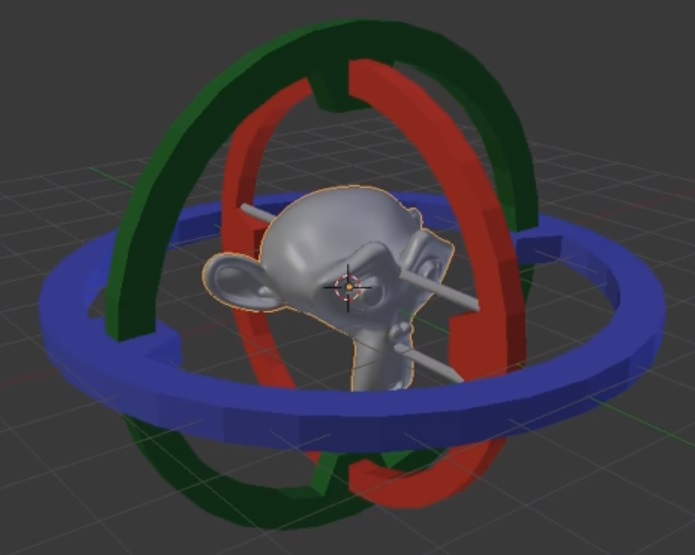
\includegraphics[width=.9\linewidth]{Figures/euler-1.jpg}
  \caption{Posizione neutra}
  \label{fig:sub1}
\end{subfigure}%
\begin{subfigure}{.5\textwidth}
  \centering
  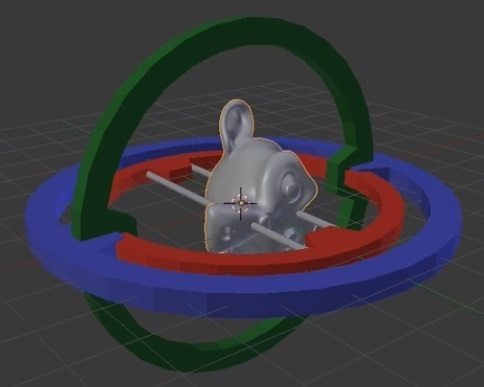
\includegraphics[width=.9\linewidth]{Figures/euler-2.jpg}
  \caption{Gimbal lock, l'asse X e Z sono allineati}
  \label{fig:sub2}
\end{subfigure}
\decoRule
\caption[Rotazione euleriana]{Rappresentazione di rotazione euleriana attraverso un giroscopio a tre assi}
\label{fig:euler1}
\end{figure}

Concettualmente è la più intuitiva di tutte: utilizza 3 assi di rotazione (X, Y, Z) ed il funzionamento è analogo a quello di un giroscopio. ogni asse offre un DOF, quindi sono possibili rotazioni con 3 DOF. Tuttavia sono necessarie due accortezze: 
\begin{enumerate}
    \item ordine degli assi;
    \item gimbal lock problem.
\end{enumerate}
L'ordine degli assi è decisivo, in quanto quello più interno dipende dalla rotazione di quelli esterni. Di conseguenza ruotando gli assi in un ordine diverso da quello specificato porta a risultati diversi da quello atteso. In più, interpolazioni tra diversi orientamenti, possono a loro volta risultare non gradevoli, poiché la rotazione viene spezzata in 3 movimenti.

Il problema del gimbal lock \parencite{anticz16}, in italiano blocco cardanico, sorge dall'allineamento di due assi: quello più interno e quello più esterno. Ne deriva che ruotano uno di questi 2 assi si ottiene la stessa rotazione, perdendo quindi un DOF.
È quindi importante scegliere l'ordine degli assi in maniera tale che il primo e il terzo non risultino mai allineati.

Per ovviare a questo problema può essere conveniente bloccare uno degli assi in una posizione fissa. Per questo motivo, la forma Euleriana è meglio utilizzata nelle giunture con 1 o 2 DOF.

\subsection{Quaternione}
\begin{figure}[ht]
\centering
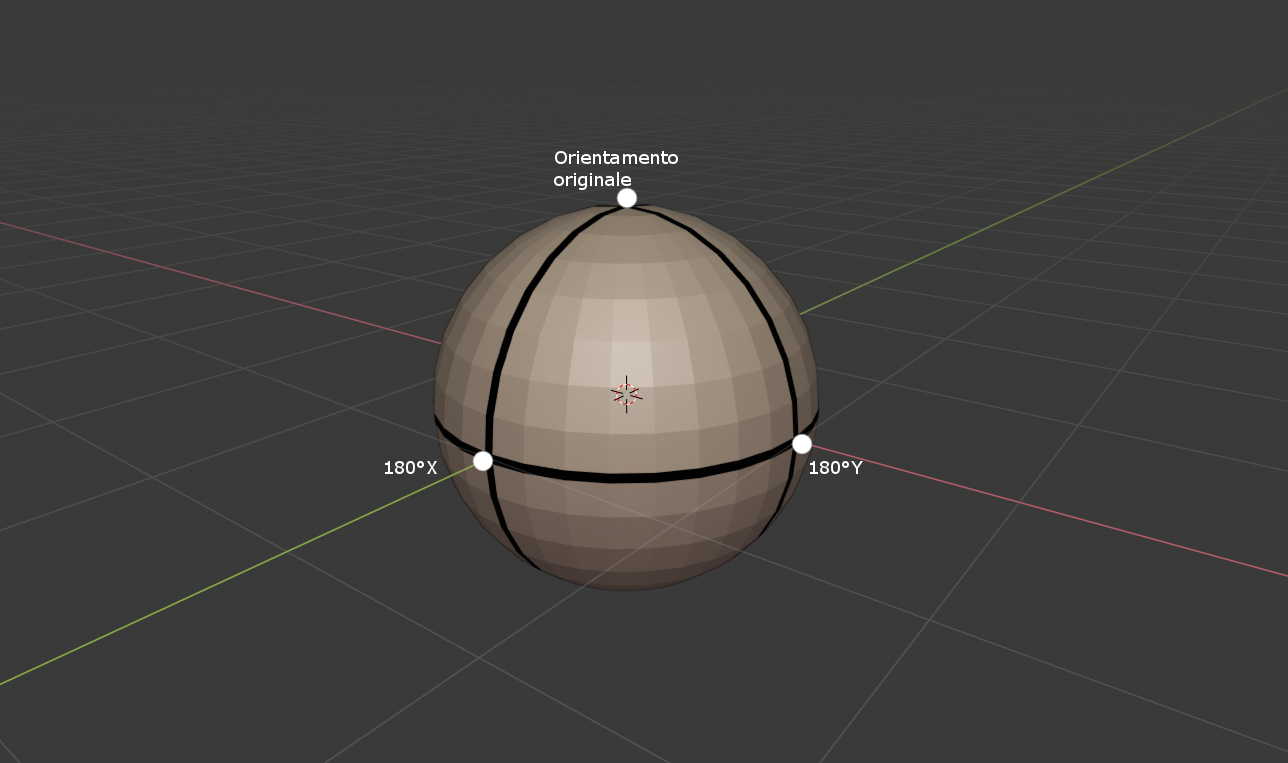
\includegraphics[width=.8\textwidth]{Figures/3d-sphere}
\decoRule
\caption[Quaternione 2D]{Rappresentazione di un quaternione 2D su una sfera 3D}
\label{fig:quater}
\end{figure}
In contrasto a quanto appena visto, la forma di quaternione è concettualmente complessa, ma in pratica diventa molto utile e senza molti dei difetti della controparte Euleriana.

I principali benefici della rappresentazione a quaternione includono l'eliminazione del gimbal lock. Infatti è presente una componente in più, ma ciascuna componente non rappresenta un asse quanto piuttosto l'orientamento dell'oggetto ruotato intorno a quell'asse. La quarta componente serve quindi a definire la posizione neutra.

L'interpolazione risulta diretta e dolce, infatti il movimento non è spezzato sui diversi assi e l'ordine di questi non è importante. Infine rende comodo calcolare una rotazione opposta semplicememte invertendo il segno della componente W.

Per rendere tutto ciò possibile servono 4 componenti (X, Y, Z, W), come già detto in precedenza, uno per la posizione originale più una per la rotazione su ogni asse. Se si prende il caso di rotazioni su due assi si può immaginare che queste 3 componenti siano 3 punti su una sfera, come mostrato in Figura \ref{fig:quater}. Ogni altra rotazione è data dall'interpolazione di questi tre punti.

La ragione per cui i due punti sulla sfera rappresentano una rotazione di 180\textdegree\ anziché 90\textdegree\ e resa necessaria siccome altrimenti questi due punti coinciderebbero nel punto più basso della sfera. Come effetto aggiuntivo possiamo rappresentare rotazioni fino a 720\textdegree\ ed ogni orientamento equivale a due possibili rotazioni dando all'animatora l'abilità di decidere in che verso ruotare l'oggetto durante un'animazione. 

\subsection{Matriciale}
Quest'ultima è probabilmente la rappresentazione più ottimale in termini di flessibilità, in quanto permette di rappresentare anche traslazioni, scalature e altre trasformazioni come \emph{shear}. È, infatti, la rappresentazione che blender utilizza internamente \parencite{blendApi, nat2012rig} poiché quella che offre la maggior flessibilità. L'unico difetto è che, come la rappresentazione sotto forma di quaternione, non mantiene l'informazione sul percorso della rotazione. Infatti è ancora più simile a una delta-rotazione (i.e. differenza di orientamento), rispetto ad un quaternione poiché copre una rotazione di soli 360\textdegree, rispetto ai 720\textdegree\ del quaternione. 


\section{Animazione di un corpo umano}
\section{Animazione facciale}

